\documentclass[a4paper, 12pt]{article}
\usepackage[utf8]{inputenc}
\usepackage{graphicx}
\graphicspath{ {images/} }
\usepackage[a4paper,left=1.5in,right=1in,top=1in,bottom=1in]{geometry}

\usepackage{tikz}
\usetikzlibrary{positioning,shapes,fit,arrows}
\definecolor{myblue}{RGB}{56,94,141}
\usepackage{fancyhdr}
\usepackage{booktabs}
\usepackage{mathtools}
\usepackage{amsmath}
\usepackage{etoolbox}
%\apptocmd{\thebibliography}{\csname phantomsection \endcsname \addtocontentsline{toc}{chapter}{\bibname}}{}{}
\usepackage{caption}
\usepackage{float}
\floatstyle{boxed} 
\restylefloat{figure}
\pagestyle{fancy}
\fancyhf{}
\fancyhead[LE,RO]{\footnotesize \center Using Data Sampling for Credit Card Fraud Detection on imbalanced Dataset. }
\fancyfoot[CE,CO]{ \raggedright{P:F-SMR-UG/08/R0} }
\fancyfoot[LE,RO]{\thepage}

\begin{document}
 
\begin{titlepage}
    \begin{center}
        \vspace*{1cm}
        
        \large
                \textbf{Pune Institute of Computer Technology}	
                \linebreak
		\textbf{Dhankawadi, Pune}
        \vspace{0.5cm}
                        \linebreak
                        \linebreak
        \textbf{A SEMINAR REPORT }
        \linebreak
        \textbf{ON }
        \linebreak
        \vspace{0.5cm}
        \large
        \\Using Data Sampling for Credit Card Fraud Detection on imbalanced Dataset. 
        \linebreak
        \linebreak
		
		%\vspace{0.2cm}
		\textbf{SUBMITTED BY}
		\vspace{1cm}
		
        \textbf{ Aamir Miyajiwala }
        \\ Roll No. 31401
        \\ Class TE 4
        \linebreak
        \linebreak
		        
        \textbf{\large{Under the guidance of}}
		\linebreak
	    Prof. A.A.Chandorkar
		\linebreak
      %  \vfill
        
        
        
        \vspace{0.8cm}
        

        
\includegraphics[scale=0.6]{./pict}   
        
        \Large
        DEPARTMENT OF COMPUTER ENGINEERING\\
%        \textbf{Pune Institute of Computer Technology}	
%		\textbf{Dhankawadi, Pune}
%		\linebreak
		\textbf{Academic Year 2020-21}
        
    \end{center}
\end{titlepage}
\pagebreak
%2
\begin{titlepage}
\begin{center}
	
\includegraphics[scale=0.6]{pict} 
	\linebreak
	\Large
        DEPARTMENT OF COMPUTER ENGINEERING\\
        \textbf{Pune Institute of Computer Technology}
		\linebreak
		\textbf{Dhankawadi, Pune-43}
		\vspace{0.8cm}
		\Large
		
	    \textbf{CERTIFICATE}
	    		\linebreak
	    \linebreak
		This is to certify that the Seminar report entitled
        \linebreak
		\linebreak
		\large
		\textbf{“Using Data Sampling for Credit Card Fraud Detection on imbalanced Dataset.”}
		\linebreak
		\linebreak
		Submitted by
		\linebreak
		Aamir Miyajiwala \hspace{10mm}   Roll No. 31401 \linebreak
		\linebreak
		has satisfactorily completed a seminar report under the guidance of Prof. A.A.Chandorkar  towards the partial fulfillment of third year Computer Engineering Semester II, Academic Year 2020-21 of Savitribai Phule Pune University. 
		\linebreak
		\linebreak
		\linebreak
		\linebreak
		\linebreak
		\begin{table}[h]
		\begin{tabular}{ccc}
		Prof. A.A.Chandorkar    &                        &  \hspace{52mm} Prof. M.S.Takalikar\\
		Internal Guide      &                     &    \hspace{52mm} Head \\
		          &                         &       \hspace{47mm} Department of Computer Engineering \\
                    &                       & \hspace{52mm} 
		\end{tabular}
		\end{table}
		\end{center}
Place:PICT,Pune
Date:26/05/2021

\end{titlepage} 

\pagenumbering{Roman}
\section*{ACKNOWLEDGEMENT}

\hspace{0.5cm} I sincerely thank our Seminar Coordinator Prof. B.D.Zope and Head of Department Prof. M.S.Takalikar
for their support.
\vspace{0.25cm}
\par I also sincerely convey my gratitude to my guide Prof. A.A.Chandorkar, Department of Computer Engineering for her constant
support, providing all the help, motivation and encouragement from beginning till end to make this seminar a grand success.
\vspace{0.25cm}
\par 

\newpage
\tableofcontents

\newpage
\listoftables
\listoffigures

\newpage

\section*{Abstract}
E-Commerce and the move towards cashless transactions has resulted in a 
significant increase in Debit/Credit Card usage. Consequently, this has resulted in 
a quantum increase in fraudulent transactions. Online fraudulent activities cost the 
global economy billions of dollars each year. Detecting and preventing anomaly 
cases like fraudulent activities is an important task for banks, insurance companies 
and small businesses.
\par 
One major problem in building a predictive model for 
anomaly detection , is the scarcity of anomalous or fraudulent data records in 
comparison to non-anomalous or non-fraudulent data which makes training 
imbalanced which will affect the classifier’s performance in bad way making it 
biased. 
\par
This work explores the use of predictive analytics for detecting anomaly 
cases by mitigating the problem of imbalanced datasets using sampling and data 
augmentation techniques. This approach can be adapted to other domains also 
where anomalous data is scarce.
  
\section*{Keywords}
Predictive Analytics,imbalanced dataset, anomaly detection,credit card..
\newpage
\pagenumbering{arabic}
\begin{center}
\section{INTRODUCTION}
\end{center}
\par
In today's world online payments and transactions have increased significantly due to the rapid development of e-commerce. Consequently this has led to a significant increase in anomalous behaviour leading to fraudulent activities.Majority of these transactions are made using Credit or Debit cards which seem to be secure, however, fraudsters are becoming more and more intelligent and can access the financial records of customer's details internally without getting caught.This give rise to the need of automated and effective  fraud detection methods which leverage the use of Machine Learning and Predictive analytics.
 \\ 
 
\par
Machine Learning algorithms are being used extensively to tackle this problem due to their ability to learn patterns of fraudulent data from historical records and detect them in future transactions.They work faster than humans can and are scalable i.e. they are adaptable for large datasets also. Due to these merits ,most credit card fraud detection approaches make use of machine learning. At present, machine learning has many approaches to solve credit card fraud detection, including unsupervised, supervised and semi-supervised learning; out of which supervised learning is the most popular due to the rise in big data technology.
\\

\par 
Frauds can be of different types and can take place in different ways and hence the classification models need to be dynamic in nature to detect the possibility of a fraud.Hence, during the learning phase of the predictive model we need to train it on various fraudulent observations for it to discern a pattern and perform efficiently.However, a significant problem faced while building a fraud detection system is the lack of fraudulent or anomalous data present in the dataset.Number of positive cases (fraudulent) is much lesser than number of negative cases which leads to the problem of imbalanced classification. This impacts the learning phase of the model drastically and therefore it's performance.Imbalanced classification causes the model to become biased,i.e. it will be inclined to classify almost every transaction as a non-fraudulent transaction.As the model becomes biased it will treat potential fraudulent observations as noise and discard it.This contradicts the purpose of building a fraud detection model.
\\

\par 
Hence, to build an efficient model, several data augmentation techniques need to be tried out and leveraged.Data augmentation is creating synthetic data from minority samples which mimic the beahviour of the minority samples.This will help in creating a balanced dataset and hence remove bias from the model improving its performance.Depending on the dataset one will need to experiment with different techniques to determine which works best.
\\




\newpage
\begin{center}

\section{MOTIVATION}

\end{center}

\hspace{1cm}
In recent times, online payment has become very convenient and has been adopted widely especially because of the rapid rise in e-commerce. It facilitates contactless payment and can be carried out anywhere. Due to this significant amount of transactions take place each day and large amount of user information is recorded which is susceptible to data breaches by fraudsters,leading to fraudulent activity. \\

\hspace{1cm} Anomalous and fraudulent data is getting common so detecting them has become a major task. Apart from normal available patterns in data new patterns are to be detected which brings a challenge for machine learning. Efficiency of detection and dynamic detection over data is also a challenge.
\\

\hspace{1cm} Thus, for effective counter measure for detecting or rather preventing fraud ,we need to apply the right data augmentation technique for the model to recognize fraudulent activity and perform well during realtime detection.\\

\newpage
\begin{center}

\section{LITERATURE SURVEY}

\end{center}

The Following table shows the literature survey by comparing techniques propose in various references:

\begin{center}
\begin{flushleft}

\begin{table}[h!]
 \caption{Literature survey}
 \begin{tabular}{|l|l|c|l|l|l|}
\hline
 No.
 & Publication 
 & Technique  
 & Model 
 & Dataset  \\ 
 \hline
 1 
 & \begin{tabular}[c]{@{}l@{}}Using\\ Variational\\ Auto Encoding \\in Credit Card\\ Fraud Detection \end{tabular} 
 & \begin{tabular}[c]{@{}l@{}}Oversampling using\\1. SMOTE \\2. GAN\\3.Variational\\Autoencoder\end{tabular}
 & \begin{tabular}[c]{@{}l@{}}Baseline \\ANN\\model  \end{tabular}     
 & \begin{tabular}[c]{@{}l@{}}European \\Credit Card\\ Holder  \end{tabular} \\ \hline

2 &\begin{tabular}[c]{@{}l@{}}Influence of \\Optimizing \\XGBoost \\to handle \\Class 
Imbalance \\in Credit Card\\ Fraud Detection\\
Learning
 \end{tabular}  
   
 &\begin{tabular}[c]{@{}l@{}}Oversampling using:\\
 1.SMOTE\\ 2.ADASYN \\3.NearMiss\\ 4.SMOTETomek
 \end{tabular}  
 & \begin{tabular}[c]{@{}l@{}}XGBoost \end{tabular}    & \begin{tabular}[c]{@{}l@{}}1.IEEE-CIS\\2.European\\Credit Card\\Holder.\end{tabular}\\
 \hline

3 &\begin{tabular}[c]{@{}l@{}}A Predictive\\ Analytics\\ Framework to \\Anomaly 
Detection

 \end{tabular}  
  
 &
 \begin{tabular}[c]{@{}l@{}}1.Oversampling\\ 2.Mini-Batch\\ Under-Sampling\\(Proposed Method)

 \end{tabular}  
 & \begin{tabular}[c]{@{}l@{}}Random Forest\\ with Feature \\selection\\ techniques.\end{tabular}     & \begin{tabular}[c]{@{}l@{}}European\\Credit Card\\Holder\end{tabular}\\
 \hline
 4 &\begin{tabular}[c]{@{}l@{}}Synthetic \\oversampling\\ with the \\majority class:\\ A
new perspective\\ on handling \\extreme imbalance

 \end{tabular}  
  
 & \begin{tabular}[c]{@{}l@{}}1.SWIM \\(proposed method)\\2.Random Oversampling\\3.Random Undersampling
 \end{tabular}  
 & \begin{tabular}[c]{@{}l@{}} Naıve Bayes\\Decision Trees\\SVM\\Multilayer\\Perceptron  \end{tabular}   
 & \begin{tabular}[c]{@{}l@{}}26 \\Benchmark\\ Datasets. \end{tabular}\\\hline

 \end{tabular}

\end{table}                             


%\\
%\\


\end{flushleft}
\end{center}

\newpage
\begin{center}
\section{A SURVEY ON PAPERS}
\end{center}
\subsection{Using Variational Auto Encoding in Credit Card Fraud Detection}
\hspace{1cm}This paper proposes a novel oversampling method based on Variational automatic encoding,combined with deep learning techniques to solve the problem of imbalanced classification often encountered while building fraud detection systems.Their approach involves bridging the gap between the fraudulent and non-fraudulent category of data by developing a framework.The framework will use oversampling of fraudulent data into the original dataset thereby augmenting it.The framework contains a sampling module attached to a baseline neural network model. The sampling module contains GAN,VAE and SMOTE.The classifier is trained with data augmented using these three different models in the sampling module and the performance of each combination is assessed.Their experimental results show that the performance of the baseline classifier was the best when fraudulent data was oversampled using VAE where the increase in samples was 0.5 times the number of original fraudulent cases in the training set.It was also determined that the recall values of SMOTE and GAN were more than VAE and since this comes under the category of supervised learning ,the VAE model could perform poorly when dealing with novel fraud data.


\subsection{Influence of Optimizing XGBoost to handle Class Imbalance in Credit Card Fraud Detection Learning.}
\hspace{1cm}  
XGBoost is a very popular model and one of the favourites of the Kaggle community, used for classification and regression problems.XGBoost is an effective machine learning model, even on datasets where the class distribution is skewed.This paper focuses on optimizing XGBoost model(hence the name OXGBoost) to perform classification of fraudulent and non-fraudulent data without the use of resampling techniques.The parameters of XGBoost are tuned using RandomizedSearchCV. This optimized model is comapred with normal XGBoost model combined with sampling techniques over two credit card fraud datasets. Experimental results show that there was no increase in performance when XGBoost was integrated with sampling techniques whereas the OXGBoost model had a boost in performance and could classification of skewed datasets without the need of data sampling techniques.


\subsection{A Predictive Analytics Framework to Anomaly Detection.}
\hspace{1cm} 
This paper adopts the use of predictive analytics for anomaly or fraud detection.Predictive analytics is a branch of artificial intelligence which learns from historical data to predict future events and give insights.This paper proposes a framework based on predictive analysis which contains three components.First being the feature selection,second being the data sampling technique and third being the predictive model being used.The framework follows a pipeline where once the data is collected and preprocessed, the framework feeds into the feature selection module,and after that into the predictive model module where the training takes place.During the training process, the problem of imbalanced classification is mitigated by performing data sampling techniques.This paper uses random oversampling and a novel method of Mini-Batch Under Sampling to balnce the dataset.The feature selection methods are used with Random Forest along with different sampling techniques where it is found that oversampling gives the best result. 


\subsection{Synthetic oversampling with the majority class: A new perspective on handling extreme imbalance.}
\hspace{1cm} This paper  starts with describing the problem of imbalanced classification and how it can be resolved using oversampling of minority class.However, in the case of extreme imbalance, the minority class is too sparse and rare, and hence , does not contain enough information to perform oversampling. For this reason,they explore the case of extreme imbalance and come up with a solution of utilizing the distributional information in majority class to augment the minority class.With this in mind they propose a novel method of oversampling called SWIM(Synthetic oversampling with the Majority).This unique method focuses on generating the minority instances in regions that have similar density with respect to the majority class and they should be neighbouring the original minority instances.SWIM was tested on 26 benchmark datasets from different domains and comapred with alternative sampling techniques.Their experimental results showed that SWIM is superior to other alternative techniques and outperformed them in 23 out of the 26 datasets.




\newpage
\begin{center}
\section{PROBLEM DEFINITION AND SCOPE}
\end{center}

\subsection{Problem Definition}

\hspace{1.5cm} To design a fraud detection system by using the suitable the right data sampling technique to prevent classification imbalance and increase efficiency of fraud detection.

\subsection{Scope}

\hspace{1.5cm} Fraud Detection is an important study for research and various methods are being developed to tackle it. Due to the scarcity of fraudulent data in a dataset we need to perform operations on data like oversampling the minority class or undersampling the majority class for the model to recognize a pattern of fraudulent activity. \\

\hspace{1.5cm} For the above purpose it is necessary to select the right data sampling technique and machine learning model to create a well balanced dataset and prevent the model from becoming biased.

\newpage
\begin{center}
\section{DIFFERENT DATA SAMPLING TECHNIQUES.}
\end{center}
\subsection{Oversampling}
\par 
\hspace{1cm}
Oversampling is used to generate examples of minority class in the dataset.It is also called as data augmentation.
\par
\subsubsection{SMOTE}
\hspace{1cm}
This is a type of data augmentation technique for the minority class and is referred to as the Synthetic Minority Oversampling Technique, or SMOTE for short.It is one of the most widely used approach for oversampling the minority class in a dataset.It works by selecting a random sample from the minority class and finds k nearest neighbours or that sample.Randomly a neighbour is selected out of the k neighbours and a synthetic example is created at a randomly selected point between the two examples in the feature space.
\par
\subsubsection{ADASYN}
\hspace{1cm}
The Adaptive Synthetic Sampling Method for Imbalanced Data, or ADASYN for short builds on the methodology of SMOTE,by shifting the importance of the classifications boundary to those minority classes which are difficult. ADASYN uses a weighted distribution for different minority class examples according to their level of difficulty in learning,where more synthetic data is generated for minority class examples that are harder to learn.
%\\
%\\
\subsection{Undersampling}
\par
\hspace{1cm}
Undersampling is the technique used for reducing the number of samples of majority class present in the dataset.
\par
\subsubsection{Random undersampling}
\par
\hspace{1cm}
This technique randomly removes samples from majority class, with or without replacement. This one of the earliest techniques used to mitigate the problem of imbalance classification.However, it may increase the variance of the classifier and may potentially discard useful or important samples.
\par
\subsubsection{NearMiss}
\hspace{1cm}
NearMiss is an under-sampling technique. It aims to balance class distribution by randomly eliminating majority class examples. When instances of two different classes are very close to each other, we remove the instances of the majority class to increase the spaces between the two classes. This helps in the classification process.To prevent problem of information loss in most under-sampling techniques, near-neighbor methods are widely used.


\newpage
\begin{center}
\section{METHODOLOGY}

\end{center}
\subsection{Workflow}
\par\\
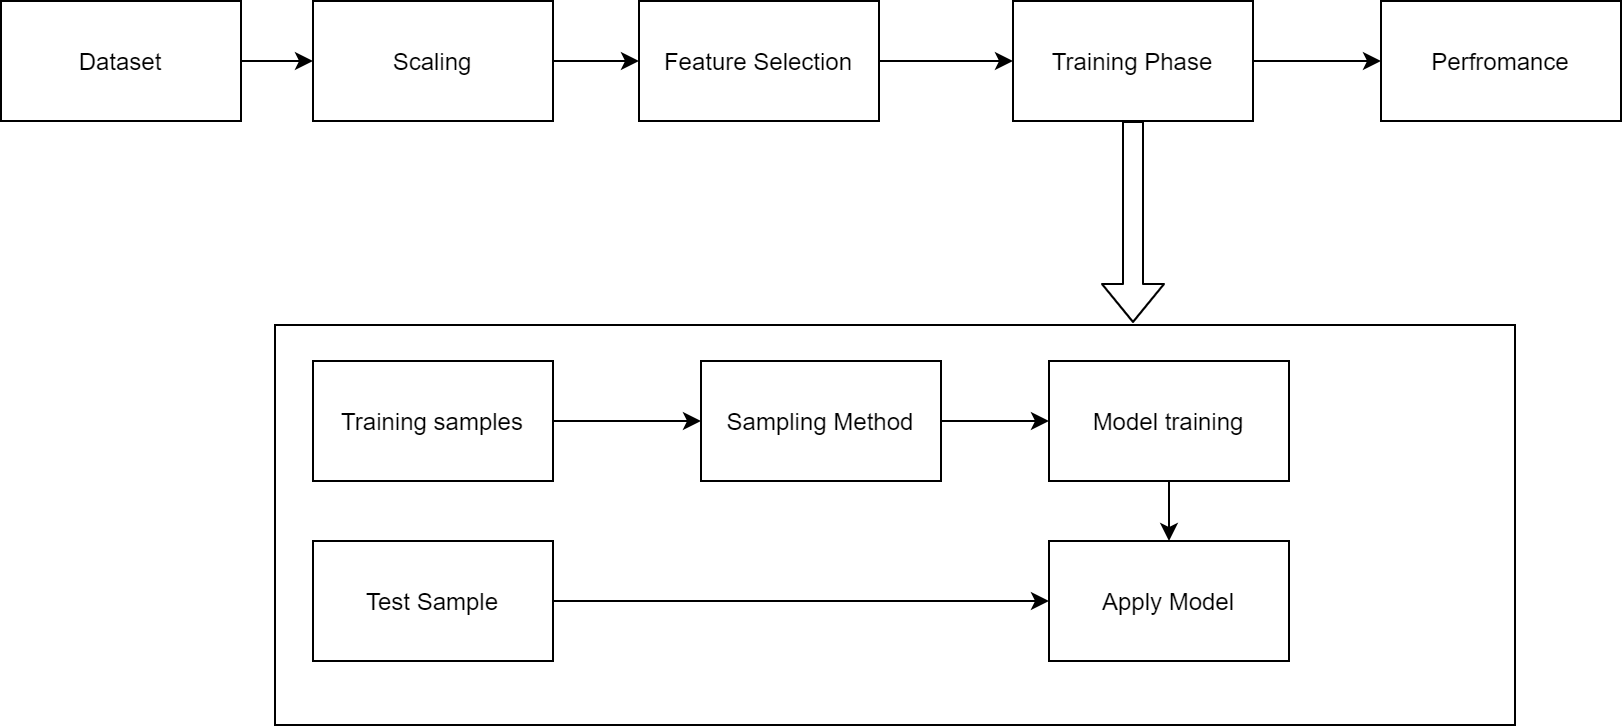
\includegraphics[width=\linewidth]{./Workflow (1)}
\par\\
\captionof{figure}{Workflow of dealing with imbalanced dataset.}
\newpage
\subsection{Mathematical model of SMOTE.}
\par
S = \{A, $x$, N, $x_k$, $x'$\}\\
Let A be the set of minority class consisting of x data points.\\

\textbf{Step1:} For each $x$ ,the \textbf{k-nearest neighbors of $x$} are obtained by calculating the Euclidean distance between $x$ and every other sample in set \textbf{A}
\\


\textbf{Step2:}The rate N is set according to the imbalanced proportion. For each $x$ in $A$, N examples (i.e x1, x2, x3, ...xn) are randomly selected from its k-nearest neighbors, and they construct the set $A_1$.\\

\textbf{Step3:}For each example $x_k$ in $A_1$ (k=1,2,3...N), the following formula is used to generate a new example:
\textbf{$x'$=$x$+rand(0,1)*($x$-$x_k$)}\\ in which rand(0,1) represents the random number between 0 and 1.

			
		

\newpage
\section{Results}
\subsection{Data}
\\
\textbf{Dataset}  : European Credit Card Holder.\\
\par
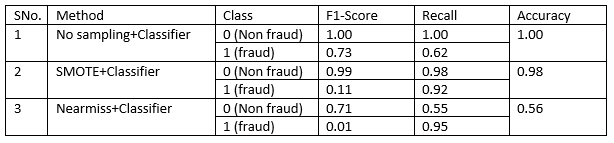
\includegraphics[width=\linewidth]{./table1}

\par\\
\captionof{table}{Classification Perfromance.}
\subsection{Implementation Results}
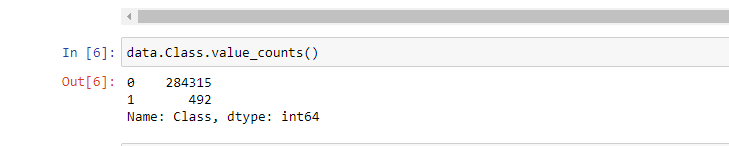
\includegraphics[width=1\linewidth]{./class}
\captionof{figure}{This is the sample count for each class.It can be observed that the number of non-fraudulent sample (class 0) is
exceedingly greater than fraudulent samples (class 1) }\\\\
\hline

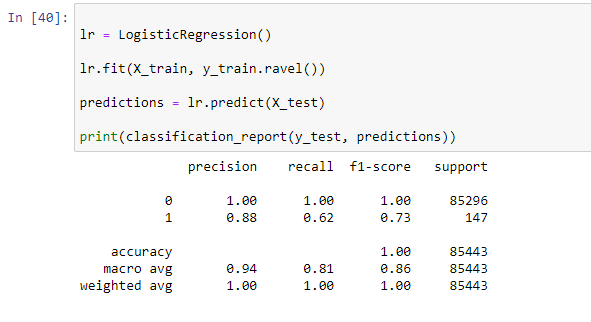
\includegraphics[width=\linewidth]{./lr}
\captionof{figure}{Performance with baseline model.Eventhough the accuracy is a 100 percent, the recall for class 1 is less.}
\hline

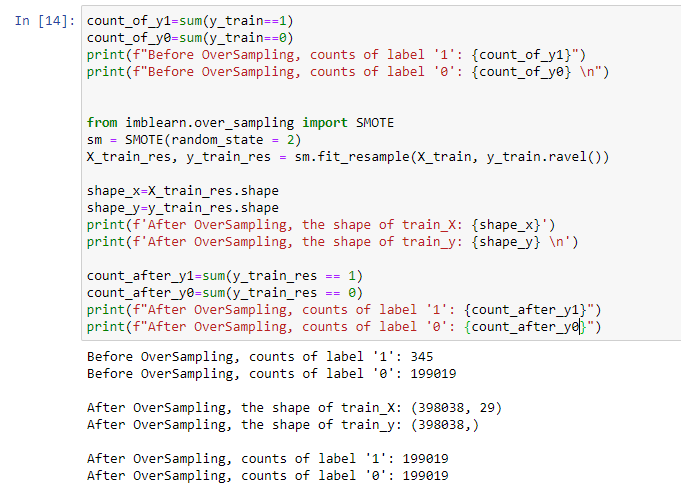
\includegraphics[width=\linewidth]{./smote}
\captionof{figure}{Applying SMOTE Oversampling technique.}
\hline

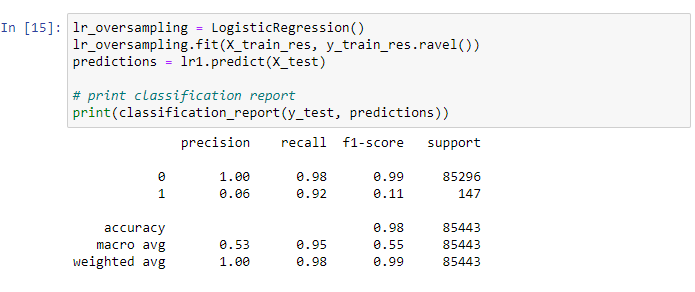
\includegraphics[width=\linewidth]{./performance_after_smote}
\captionof{figure}{Performance after oversampling with baseline model. Here we can observe that the accuracy dipped a little but the recall value for the minority class has increased.}
\hline

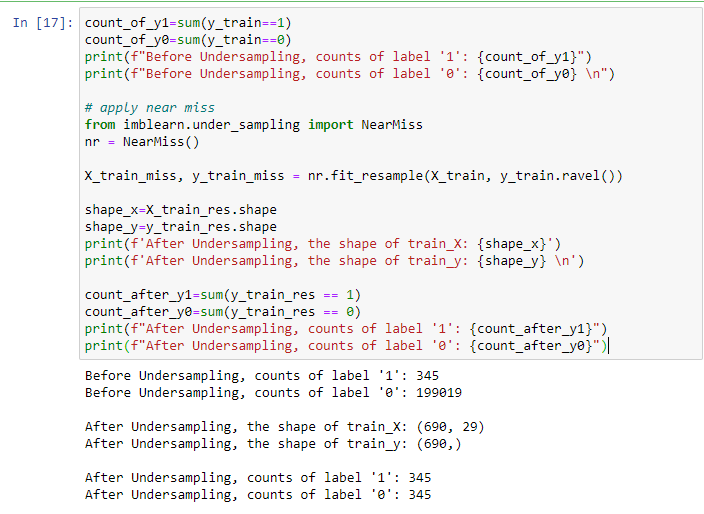
\includegraphics[width=\linewidth]{./undersampling}
\captionof{figure}{Applying Nearmiss undersampling technique}
\hline
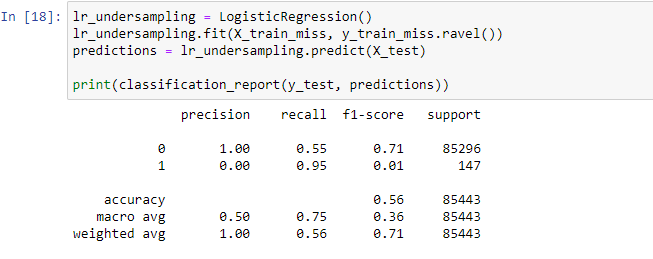
\includegraphics[width=\linewidth]{./performance_after_undersampling}
\captionof{figure}{Performance after undersampling with baseline model.Here, even though the recall value for minority class increased, the recall for majority class decreased significantly along with accuracy which shows that there has been some loss of information from majority class.}
\newpage
\begin{center}
\section{CONCLUSION}
\end{center}
\par
Fraud detection is of utmost importance and while building a system one cannot afford to let the model have any bias towards one class.Hence, it is necessary to perform data sampling techniques to create a well balanced dataset to get rid of any bias.While there are different methods of oversampling and undersampling techniques,oversampling methods have been proved to give a better classification performance.
\par
The scope of Fraud Detection is huge and data sampling can help the machine learning models learn different kinds of frauds by generating synthetic data mimicking fraudulent behaviour.
\\

\newpage
%
%\bibliography{biblio}
\addcontentsline{toc}{section}{References}
\bibliographystyle{plain}

\begin{thebibliography}{21}
\bibitem{paper1} S. Sharma, C. Bellinger, B. Krawczyk, O. Zaiane, and N. Japkowicz, "Synthetic oversampling with the majority class: A new perspective on handling extreme imbalance," in Proc. IEEE Int. Conf. Data Mining (ICDM), Singapore, Nov. 2018, pp. 447–456. .

\bibitem{paper2} H. Tingfei, C. Guangquan and H. Kuihua, "Using Variational Auto Encoding in Credit Card Fraud Detection," in IEEE Access, vol. 8, pp. 149841-149853, 2020, doi: 10.1109/ACCESS.2020.3015600.

\bibitem{paper3} C. V. Priscilla and D. P. Prabha, "Influence of Optimizing XGBoost to handle Class Imbalance in Credit Card Fraud Detection," 2020 Third International Conference on Smart Systems and Inventive Technology (ICSSIT), 2020, pp. 1309-1315, doi: 10.1109/ICSSIT48917.2020.9214206.

\bibitem{paper4} J. Wang, R. Martins de Moraes and A. Bari, "A Predictive Analytics Framework to Anomaly Detection," 2020 IEEE Sixth International Conference on Big Data Computing Service and Applications (BigDataService), 2020, pp. 104-108, doi: 10.1109/BigDataService49289.2020.00023.

\bibitem{paper5} Mohammed, Rafiq Ahmed, et al. "Scalable machine learning techniques for highly imbalanced credit card fraud detection: a comparative study." Pacific Rim International Conference on Artificial Intelligence. Springer, Cham, 2018.


\bibitem{paper6} T. Hasanin, T. M. Khoshgoftaar, J. L. Leevy, and N. Seliya, ‘‘Examining characteristics of predictive models with imbalanced big data,’’ J. Big Data, vol. 6, no. 1, p. 69, Dec. 2019.






\end{thebibliography}

\newpage
\begin{center}
\begin{flushleft}
\begin{table}[h!]
 \caption{Review Log}
 \begin{tabular}{|c|c|l|l|}
\hline
 No.& Date 
 & Points discussed
 & Suggestions given  
 \\ 
 \hline
1& \begin{tabular}[c]{@{}l@{}}$28^{th}$ February 2021\end{tabular}
& \begin{tabular}[c]{@{}l@{}}Informed guide about\\
the selected domain and\\
shortlisted papers
\end{tabular} 
& \begin{tabular}[c]{@{}l@{}}Discuss the understanding\\
of papers to finalize\\
seminar topic and base paper
\end{tabular}
\\
\hline


2& \begin{tabular}[c]{@{}l@{}}$8^{th}$ March 2021\end{tabular}
& \begin{tabular}[c]{@{}l@{}}Presented the shortlisted\\
papers and discussed their\\
understanding with guide
\end{tabular} 
& \begin{tabular}[c]{@{}l@{}}Seminar guide \\Prof. A.A.Chandorkar\\
approved a topic \\and gave a go-ahead.
\end{tabular}
\\
\hline


3& \begin{tabular}[c]{@{}l@{}}$16^{th}$ March 2021\end{tabular}
& \begin{tabular}[c]{@{}l@{}}Presented the literature\\review progress, discussed \\problem statement with\\
seminar guide.
\end{tabular} 
& \begin{tabular}[c]{@{}l@{}} Corrections in the problem\\
statement. The literature \\survey should
be thorough.

\end{tabular}
\\
\hline


 4& \begin{tabular}[c]{@{}l@{}} $11^{th}$ April 2021\end{tabular}
& \begin{tabular}[c]{@{}l@{}}Abstract Submission for \\
guide's approval
\end{tabular} 
& \begin{tabular}[c]{@{}l@{}}Topic and abstract\\
accepted by the

seminar guide
\end{tabular}
\\
\hline

 \end{tabular}

\end{table}                             


%\\
%\\


\end{flushleft}
\end{center}


\newpage

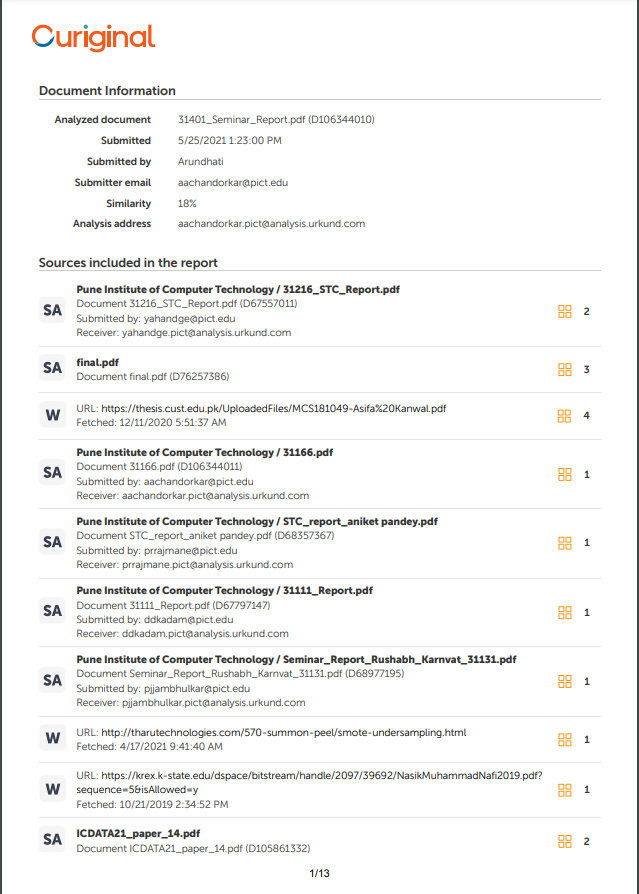
\includegraphics[width=\linewidth]{./plagiarism}
\newpage
Guide's Approval.\\
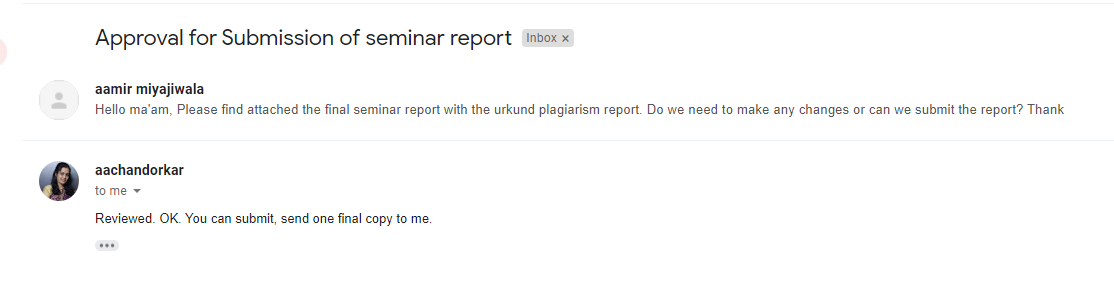
\includegraphics[width=\linewidth]{./approval}

\end{document}

